
\section{System Overview}

This chapter presents the main contribution of this thesis. It describes the proposed framework for constructing a Virtual Knowledge Graph (VKG) over a relational movie database and enabling natural language interaction through Large Language Models (LLMs). The chapter explains each stage of the framework, including data preparation, ontology design, semantic mappings, Virtual Knowledge Graph construction, and the integration of LLMs for user intent recognition, semantic querying, and recommendation support.
\section{Dataset}
The proposed framework was evaluated using a synthetic Netflix-style streaming dataset designed to simulate realistic user interactions on a video streaming platform. The dataset was selected because it provides multiple interconnected data sources that support both semantic querying and recommendation tasks.

The dataset consists of six CSV files representing the main entities and user interactions of the platform: users, movies, watch history, reviews, search logs, and recommendation logs. Together, these files contain more than 210,000 records covering user demographics, movie metadata, viewing activities, textual reviews, search behavior, and recommendation events.

Unlike real-world industrial datasets, the selected dataset is synthetic and was generated to reproduce realistic user behavior while avoiding privacy concerns. In addition, it intentionally includes missing values, duplicate records, and outliers, making it suitable for evaluating data integration and semantic querying approaches.
\section{PostgreSQL Database}
As the first implementation step, the six CSV files of the dataset were imported into a PostgreSQL relational database using pgAdmin. Each CSV file was loaded as an independent relational table while preserving the original structure of the dataset.

The resulting database consists of six interconnected tables corresponding to users, movies, watch history, reviews, search logs, and recommendation logs. Primary keys uniquely identify each record, whereas foreign keys establish the relationships between users, movies, and interaction tables.

The PostgreSQL database serves as the persistent data layer of the proposed framework. All user information, movie metadata, and interaction records remain physically stored in the relational database throughout the execution of the system.
\section{Database Schema}
The PostgreSQL database is composed of six interconnected relational tables representing the main entities and user interactions of the streaming platform. The database preserves the original relational structure of the dataset after the import process.

The main entity tables are \textbf{users} and \textbf{movies}, while the remaining tables store different types of interactions between users and movies, including watch history, reviews, search activities, and recommendation events. These relationships are established through primary and foreign keys, allowing efficient retrieval of related information.

Figure~\ref{fig:er_schema} illustrates the Entity--Relationship (ER) schema of the relational database used in this thesis.

\begin{figure}[H]
\centering
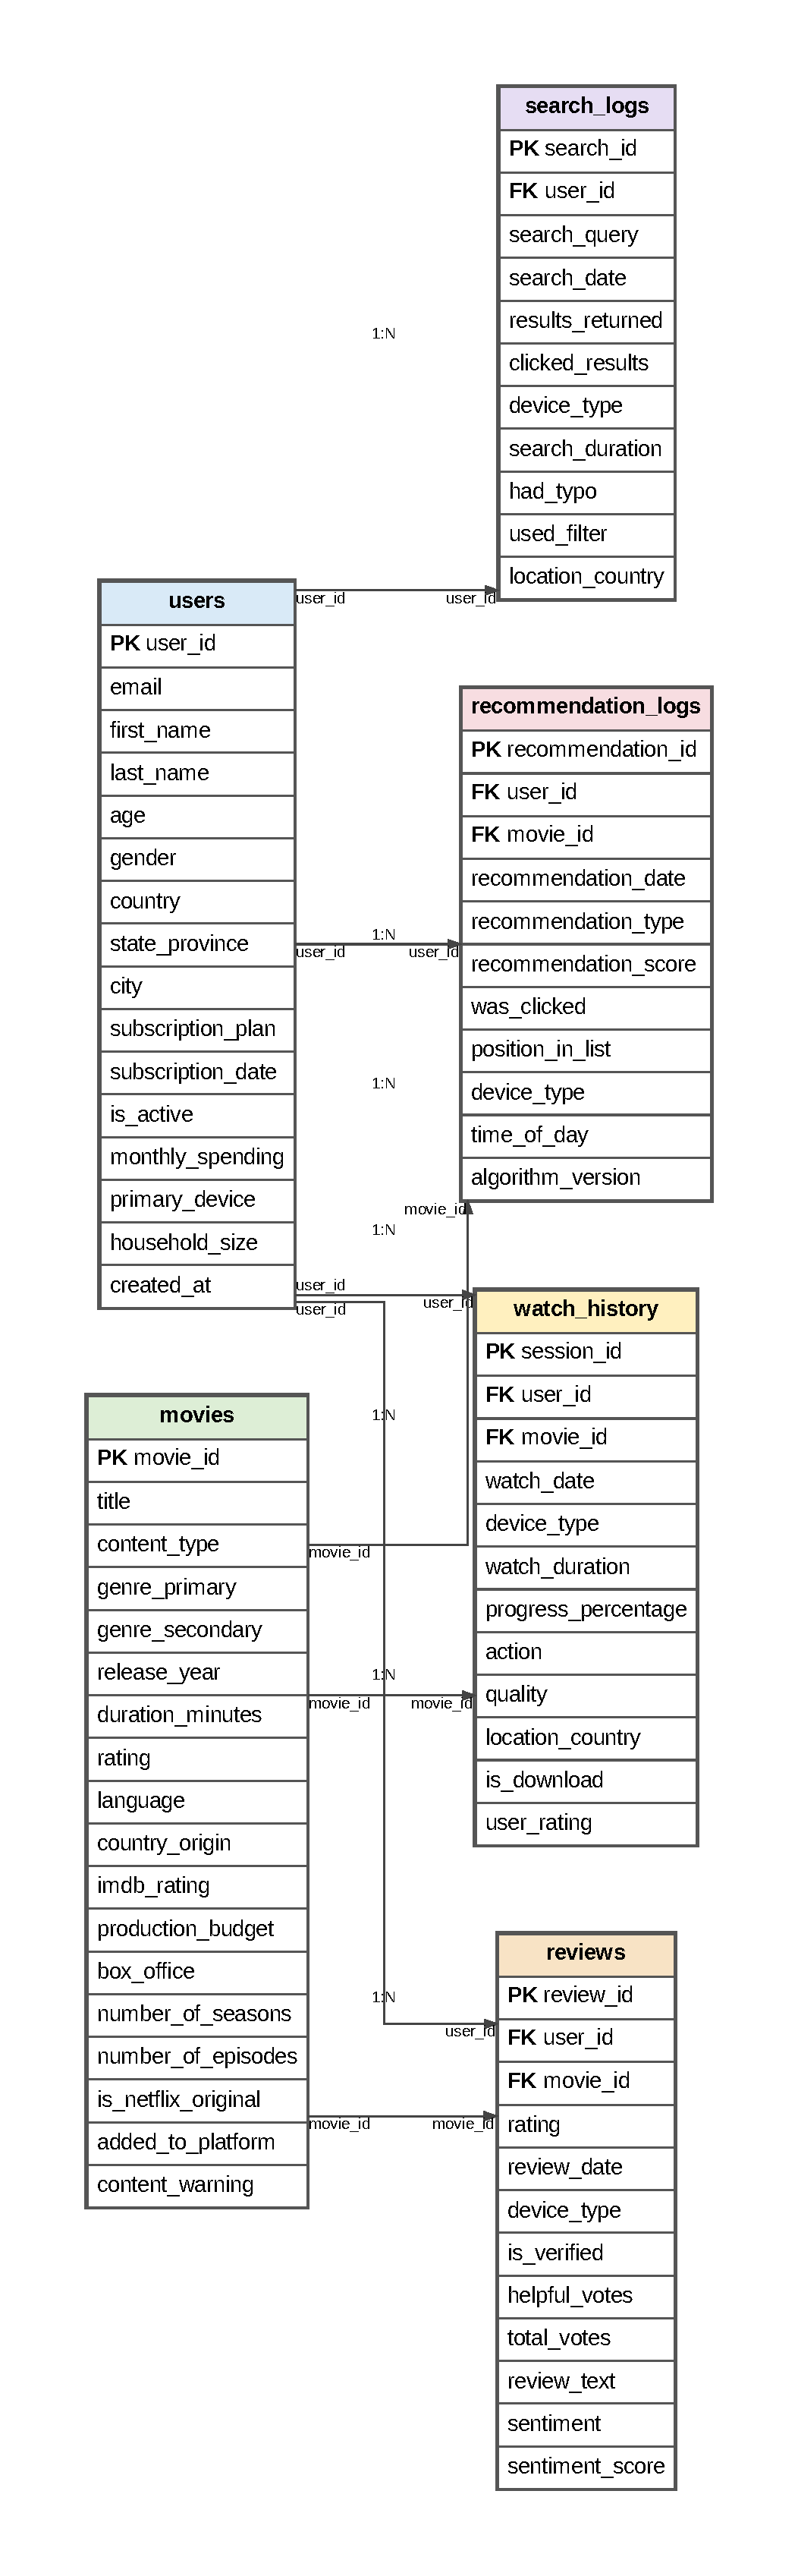
\includegraphics[width=0.95\textwidth]{sections/images/er_schema_netflix.pdf}
\caption{Entity--Relationship schema of the PostgreSQL database.}
\label{fig:er_schema}
\end{figure}
\begin{itemize}
    \item \textbf{users}: Stores demographic and subscription information.
    \item \textbf{movies}: Stores movie metadata.
    \item \textbf{reviews}: Stores user ratings and textual reviews.
    \item \textbf{watch\_history}: Records users' viewing activities.
    \item \textbf{search\_logs}: Stores users' search queries.
    \item \textbf{recommendation\_logs}: Stores recommendation events generated by the platform.
\end{itemize}
\section{Ontology Design}

After defining the relational database schema, an ontology was created to provide a conceptual representation of the movie domain. The ontology was designed using Protégé and represents the main concepts of the dataset as semantic classes and properties.

The main ontology classes were derived from the relational tables of the PostgreSQL database. In particular, classes such as \textbf{User}, \textbf{Movie}, \textbf{Review}, \textbf{WatchHistory}, \textbf{SearchLog}, and \textbf{RecommendationLog} represent the main entities and user interaction records of the streaming platform.

Object properties were used to represent semantic relationships between these classes. For example, a user can watch a movie, write a review, perform a search, or receive a recommendation. Data properties were used to describe literal values such as movie titles, release years, user demographic information, ratings, search queries, and watch duration.

The ontology does not store the original dataset records. Instead, it defines the conceptual structure used to access the relational data semantically. The actual data remain stored in PostgreSQL and are connected to the ontology through semantic mappings.
\section{Semantic Mappings}

After the ontology was designed, semantic mappings were created to connect the ontology with the PostgreSQL database. The mappings establish the correspondence between relational tables and ontology elements, allowing database records to be represented as RDF resources without physically transforming the data.

The mappings were implemented using the Ontop mapping language. Each mapping consists of an SQL query that retrieves data from the relational database and a target specification that generates RDF triples according to the ontology vocabulary.

For example, records stored in the \textbf{movies} table are mapped to instances of the \textbf{Movie} class, while database columns are associated with ontology properties through mapping assertions. Similar mappings were created for users, reviews, watch history, search logs, and recommendation logs.


\subsection{Example Mapping}

Listing~\ref{lst:movie_mapping} presents one of the semantic mappings implemented in this work. This example illustrates how data stored in the relational database are transformed into RDF triples by combining an SQL query with a target mapping defined according to the ontology vocabulary.
\begin{lstlisting}[caption={Example of the movie-basic-mapping implemented in Ontop},label={lst:movie_mapping}]
mappingId    movie-basic-mapping

target       :movie/{movie_id} a :Movie ;
             :title {title} ;
             :releaseYear {release_year} ;
             :contentType {content_type} .

source       SELECT movie_id,
                    title,
                    release_year,
                    content_type
             FROM movies
             WHERE movie_id IS NOT NULL
               AND title IS NOT NULL
               AND release_year IS NOT NULL
               AND content_type IS NOT NULL
\end{lstlisting}

The mapping shown above illustrates the basic structure of an Ontop mapping. The \textit{source} component contains the SQL query executed over the PostgreSQL database, whereas the \textit{target} component specifies how the retrieved records are transformed into RDF triples according to the ontology vocabulary. In this example, each movie is represented as an individual of the \textbf{Movie} class, while its title, release year, and content type are exposed as ontology data properties. Consequently, the relational data can be queried semantically through the Virtual Knowledge Graph without modifying or duplicating the original database.

\section{Virtual Knowledge Graph Construction}

After defining the ontology and the semantic mappings, the Virtual Knowledge Graph was constructed using Ontop. In this architecture, the data are not physically converted into RDF. Instead, they remain stored in the PostgreSQL database, while Ontop uses the ontology and mappings to expose them as a virtual RDF graph.

The Virtual Knowledge Graph connects the conceptual layer represented by the ontology with the relational data stored in PostgreSQL. When a SPARQL query is submitted, Ontop uses the mappings to translate the query into SQL and retrieves the corresponding results from the database.

This approach makes it possible to query the movie dataset at a semantic level without duplicating the original data. The resulting VKG therefore provides a unified semantic access layer over the relational database and serves as the basis for the natural language querying and recommendation components of the proposed framework.
\section{SPARQL Query Execution}

After constructing the Virtual Knowledge Graph, SPARQL queries were executed to validate both the ontology and the semantic mappings. Since the relational data are exposed as RDF through Ontop, users can formulate semantic queries without interacting directly with the PostgreSQL database.

When a SPARQL query is submitted, Ontop automatically translates it into an equivalent SQL query according to the defined mappings. The generated SQL query is then executed over the relational database, and the results are returned through the Virtual Knowledge Graph.

Several SPARQL queries were developed to verify that the ontology classes, properties, and mappings correctly represented the underlying relational data. These queries retrieve information about movies, users, reviews, watch history, search activities, and recommendation records, confirming that the semantic layer provides consistent access to the database.
\section{Natural Language Reasoning}

One of the main objectives of the proposed framework is to simplify user interaction with the Virtual Knowledge Graph. Instead of requiring users to formulate SPARQL queries, the system allows them to express their information needs using natural language.

When a user submits a request, the natural language input is first analyzed to identify its semantic meaning and determine the user's intention. This reasoning process represents the first step of the framework and allows the system to understand whether the request requires factual information retrieval or recommendation support.

By introducing a reasoning layer before query execution, the framework separates language understanding from data access. This architecture improves usability by enabling users with no knowledge of Semantic Web technologies or SPARQL syntax to interact with the underlying Knowledge Graph.
\section{Intent Detection}

After the natural language request has been analyzed, the framework performs intent detection. The purpose of this step is to classify the user's request according to the type of information required.

Two main categories of user requests are considered. The first category includes factual questions that can be answered by retrieving structured information from the Virtual Knowledge Graph. Examples include requests for movie metadata, user information, reviews, or viewing history. The second category includes recommendation-oriented requests, where the user expects personalized suggestions or analytical responses rather than direct retrieval of stored information.

This classification enables the framework to select the most appropriate processing strategy. Requests classified as factual are forwarded to the semantic querying module, whereas recommendation-oriented requests are handled by the recommendation component of the framework.
\section{Natural Language to SPARQL Translation}

For factual requests, the framework translates the interpreted natural language query into an equivalent SPARQL query. Instead of manually writing SPARQL syntax, users formulate their requests in natural language, while the framework automatically generates the semantic query required to access the Virtual Knowledge Graph.

The generated SPARQL query is executed through Ontop, which translates it into SQL according to the semantic mappings defined between the ontology and the PostgreSQL database. The query results are then returned to the user in a structured and human-readable form.

This component allows semantic querying without requiring users to understand the ontology structure, RDF representation, or SPARQL syntax, thereby improving the accessibility of the proposed system.
\section{Recommendation Module}

Not all user requests require simple information retrieval. Some requests involve recommendation tasks, such as suggesting movies that match user preferences or viewing behavior. For these requests, the framework routes the query to a recommendation module instead of directly generating a SPARQL query.

The recommendation module is designed as an independent component of the overall architecture. It can exploit information stored in the dataset, including watch history, user ratings, search activities, and movie metadata, to generate personalized recommendations.

Within the proposed framework, the recommendation component complements semantic querying by providing intelligent suggestions based on user interactions and content characteristics. The detailed implementation of this module will be extended in future developments of the system.
\section{Overall Framework Workflow}

Figure~\ref{fig:framework_workflow} summarizes the overall workflow of the proposed framework.

The process begins when a user submits a natural language request. The reasoning component analyzes the input and performs intent detection to determine the appropriate execution path. Factual requests are translated into SPARQL queries and executed through Ontop over the Virtual Knowledge Graph, while recommendation-oriented requests are forwarded to the recommendation module. Finally, the generated results are returned to the user through the application interface.

This modular architecture separates semantic data access from intelligent recommendation, making the framework flexible, extensible, and suitable for future integration with more advanced Large Language Models and recommendation algorithms.
\begin{figure}[H]
...
\caption{Overall workflow of the proposed framework.}
\label{fig:framework_workflow}
\end{figure}